% ============================================================
% Resumo CONPEEX 2026 — Edital PROEC Nº 08/2026
% Prazo: 26/06/2026 às 17h | https://23conpeex.plateia.ufg.br/
%
% INSTRUÇÕES:
%   Este arquivo gera o PDF de referência para revisão.
%   O texto do resumo deve ser colado manualmente no campo
%   "Resumo" do PLATEIA (sistema não aceita upload de PDF).
%
% Compilar: pdflatex resumo_conpeex_2026.tex
% ============================================================
\documentclass[12pt, a4paper]{article}

\usepackage[utf8]{inputenc}
\usepackage[T1]{fontenc}
\usepackage[brazil]{babel}
\usepackage{helvet}
\renewcommand{\familydefault}{\sfdefault}
\usepackage[top=3cm, bottom=2cm, left=3cm, right=2cm]{geometry}
\usepackage{setspace}
\onehalfspacing
\usepackage{booktabs}
\usepackage{graphicx}
\usepackage{float}
\usepackage{caption}
\usepackage{subcaption}
\usepackage{amsmath}
\usepackage[hidelinks]{hyperref}

\pagestyle{empty}

% ============================================================
\begin{document}

% ── Cabeçalho institucional ─────────────────────────────────
\begin{center}
  {\large\textbf{23º CONPEEX --- Congresso de Pesquisa, Ensino e Extensão da UFG}} \\[4pt]
  {\normalsize Edital PROEC Nº 08/2026 | Seminário de Iniciação à Pesquisa --- PIP --- Iniciação Científica (IC)} \\[8pt]

  % ── Título (CAIXA ALTA, ≤150 caracteres) ──────────────────
  {\large\textbf{DESENVOLVIMENTO DE FRAMEWORK ADAPTIVO PARA SELEÇÃO DE ALGORITMOS DE
  PLANEJAMENTO DE TRAJETÓRIA EM NAVEGAÇÃO AUTÔNOMA}} \\[8pt]

  {\normalsize
    Yan Santos Leite\textsuperscript{1},
    Aldo André Diaz Salazar\textsuperscript{2} \\[4pt]
    \textsuperscript{1}Engenharia Mecânica, EMC/UFG --- santosleiteyan@icloud.com \\
    \textsuperscript{2}Instituto de Informática, UFG --- aldo.diaz@ufg.br
  }
\end{center}

\vspace{0.5cm}
\noindent\rule{\linewidth}{0.4pt}
\vspace{0.3cm}

% ── Resumo ──────────────────────────────────────────────────
\noindent\textbf{Resumo:}

\noindent
Quando um robô precisa ir de um ponto a outro, ele utiliza um algoritmo de planejamento de
trajetória para decidir por onde passar. Algoritmos tradicionais, como o A*, são muito
eficientes em ambientes simples, mas perdem desempenho quando há muitos obstáculos. Já
algoritmos baseados em aprendizado de máquina lidam melhor com ambientes complexos, porém
são desnecessariamente lentos quando o caminho é livre. Na prática, a escolha do algoritmo é
feita uma única vez pelo engenheiro, independentemente do ambiente em que o robô vai operar.
A tese deste trabalho é que \textbf{escolher o algoritmo de forma adaptiva, durante a
navegação, supera métodos de escolha fixa} em ambientes heterogêneos.

A contribuição central é o $\rho$-criterion: um critério que, a cada momento, mede quantos
obstáculos há ao redor do robô e seleciona automaticamente o algoritmo mais adequado para
aquele trecho. Em espaços abertos, o cálculo analítico do A* é suficiente e rápido; em
regiões congestionadas, uma política aprendida por reforço (SAC, \textit{Soft Actor-Critic})
navega melhor. O limiar $\rho^* = 0{,}30$ que separa os dois regimes foi obtido por
experimentos: é o ponto em que um planejador passa a superar o outro e, a partir do qual,
usar mais o método aprendido quase não aumenta o sucesso --- o melhor equilíbrio entre
eficácia e custo.

Em 1.500 cenários de simulação (Monte Carlo), com modelos de planejamento calibrados a partir
da literatura, o framework adaptivo alcançou \textbf{85,3\% de taxa de sucesso}, contra 76\%
do melhor método fixo, ficando a apenas \textbf{2,2\%} de um seletor ideal --- aquele que
conhece o ambiente de antemão. O estudo dos algoritmos clássicos também justificou a escolha
do A*: o Floyd-Warshall, por exemplo, leva 39 segundos num mapa de médio porte, inviável em
tempo real.

Esses resultados confirmam a tese nesta primeira fase do trabalho; a validação com
planejadores reais em ambiente robótico (ROS2/Gazebo) está em andamento, com resultados
finais previstos para o encerramento do ciclo. Como o critério depende apenas da densidade
local, estende-se naturalmente a frotas de múltiplos robôs, direção em que o aprendizado por
reforço multi-agente se apresenta como próxima etapa.

\vspace{0.4cm}
\noindent\textbf{Palavras-chave:} planejamento de trajetória; aprendizado por reforço;
navegação autônoma; ROS2; seleção adaptativa.

\vspace{0.3cm}
\noindent\rule{\linewidth}{0.4pt}

% ── Figuras para apresentação ────────────────────────────────
\vspace{0.5cm}
\noindent\textbf{Material visual --- apresentação CONPEEX}

% ── Figura 1: Motivação e critério ──────────────────────────
\begin{figure}[H]
  \centering
  
\includegraphics[width=\textwidth]{figs/pareto/fig_pareto_boxplot_main.png}
  \caption{Justificativa formal de $\rho^*{=}0{,}30$: boxplots de taxa de sucesso por limiar
           e equações de retorno marginal. ROI$=\Delta S/\Delta f_{\text{SAC}}{=}0{,}11$~pp/pp
           em $\tau{=}0{,}30$ --- ponto Pareto-ótimo entre eficácia e custo computacional.}
  \label{fig:pareto_boxplot_conpeex}
\end{figure}

% ── Figura 2: Mapa de decisão ────────────────────────────────
\begin{figure}[H]
  \centering
  \begin{subfigure}[b]{0.48\textwidth}
    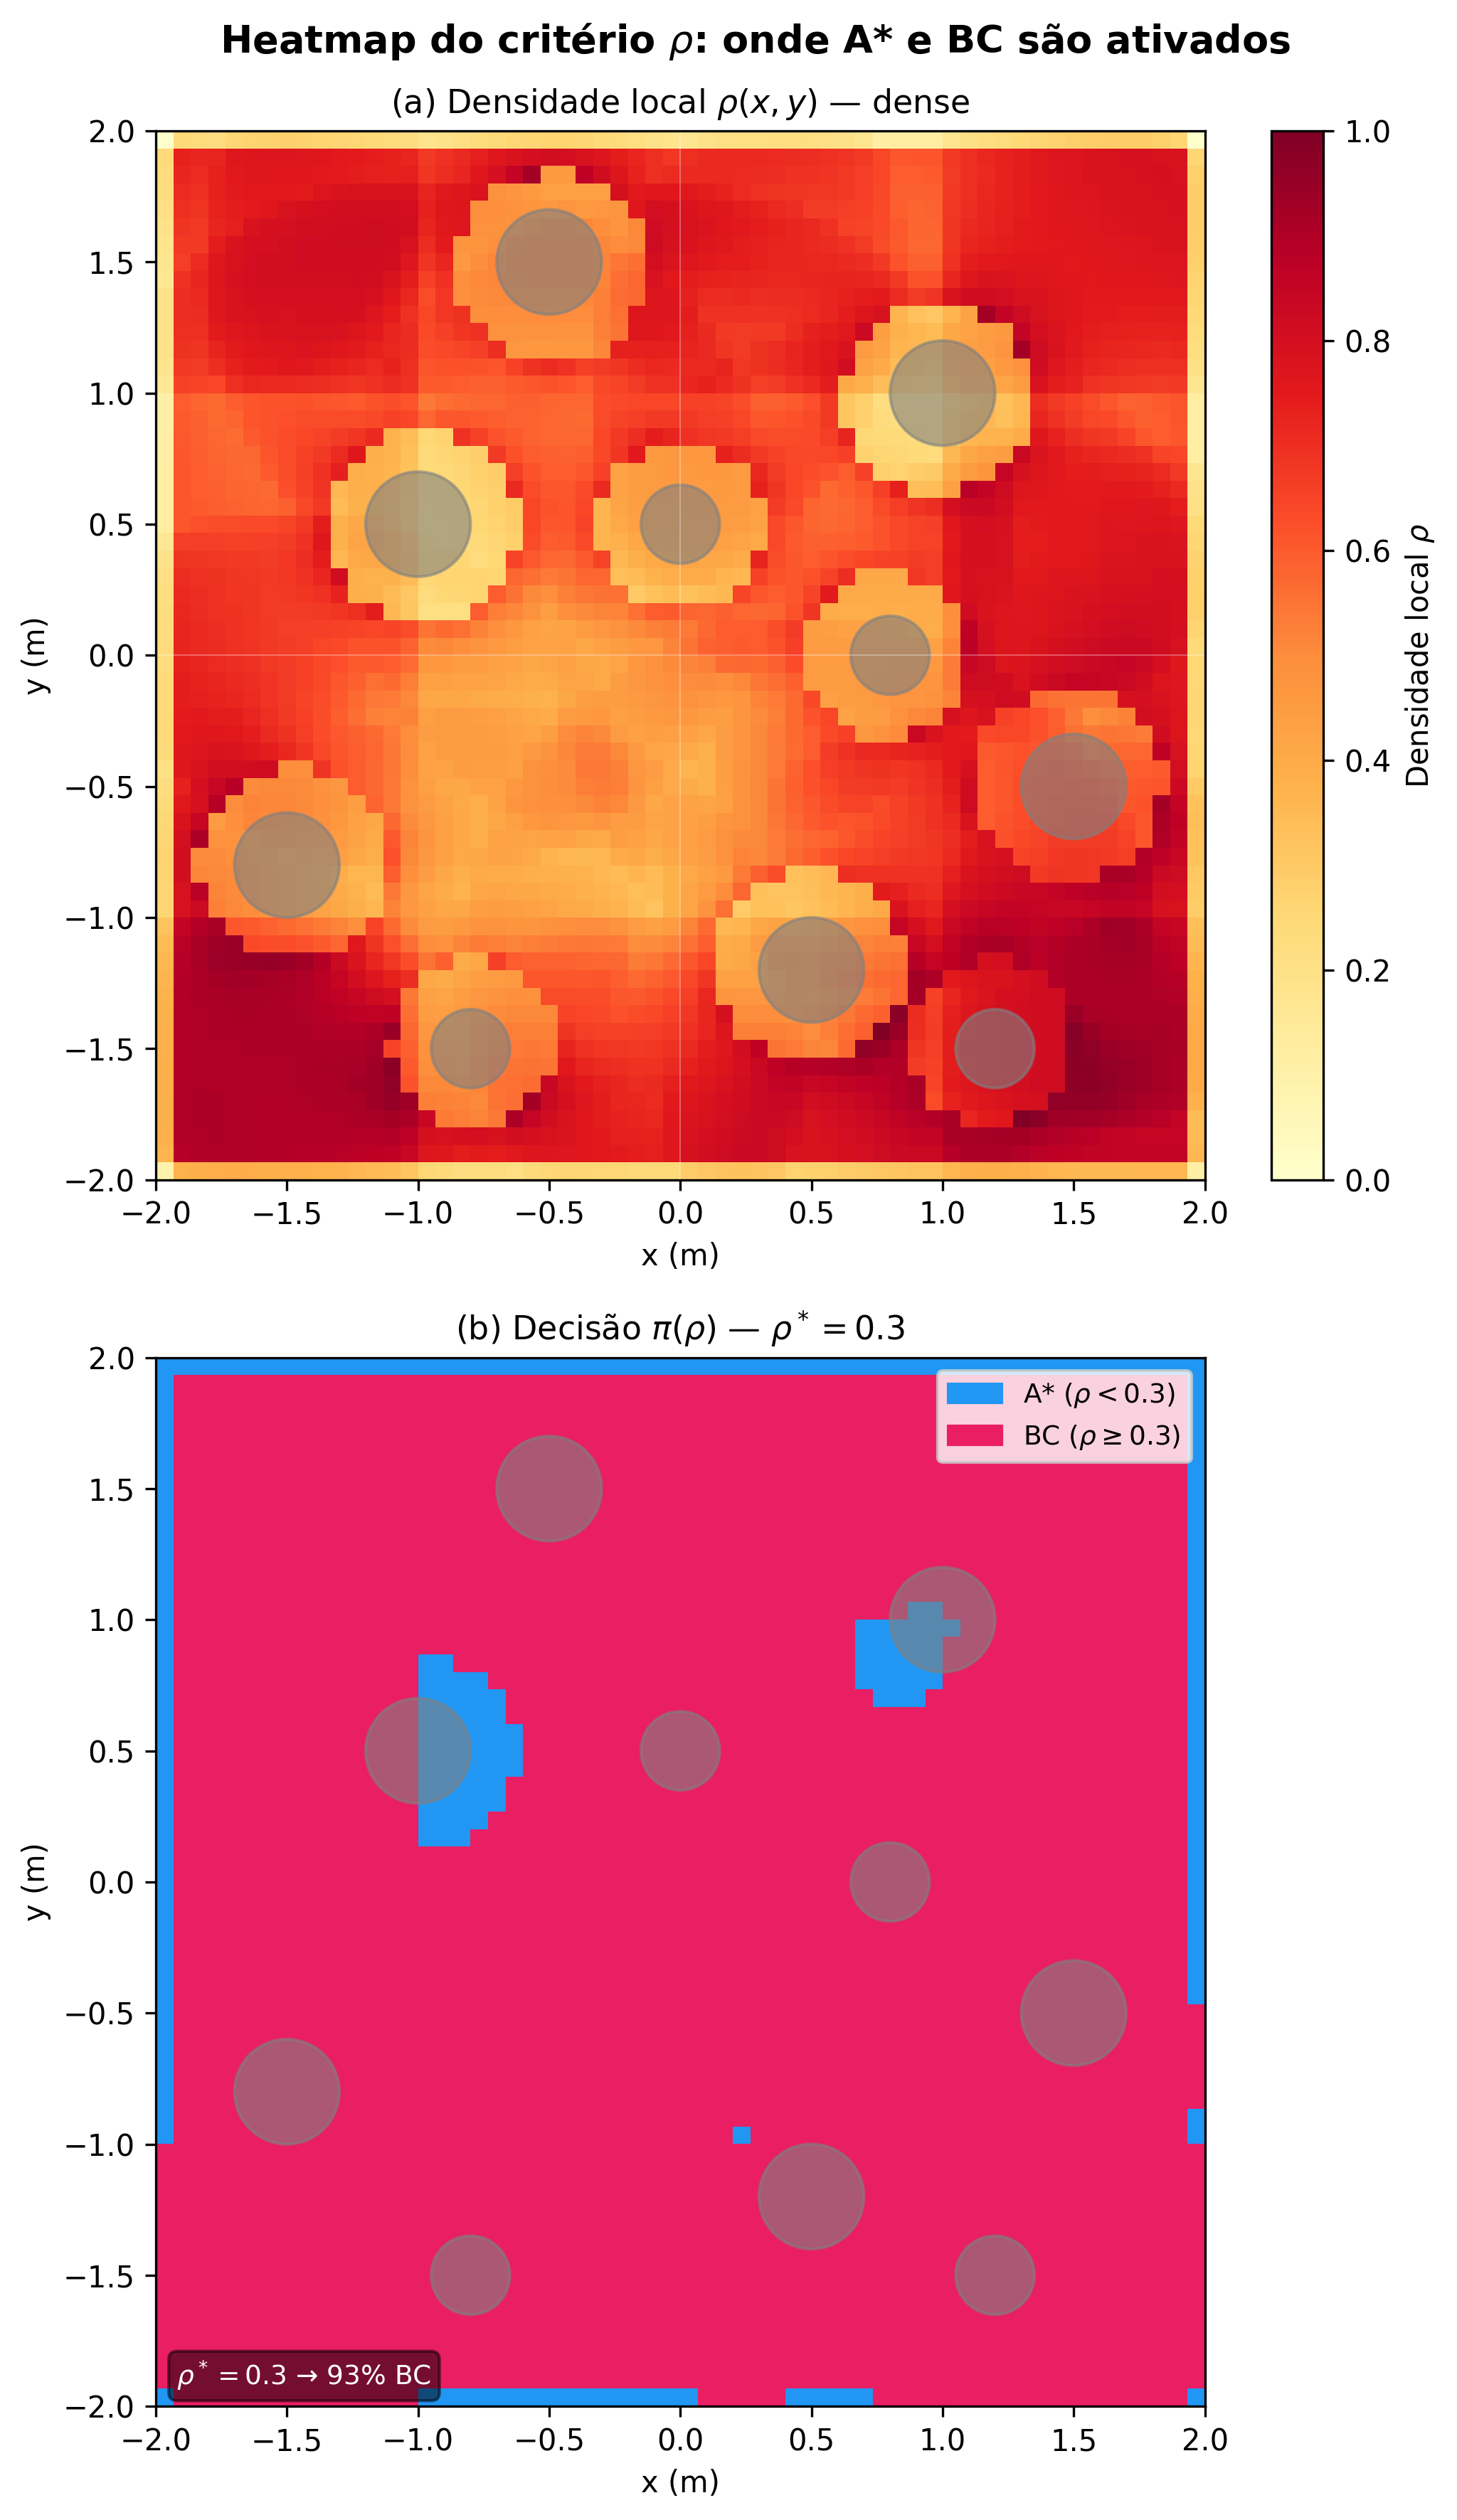
\includegraphics[width=\textwidth]{figs/2d/fig_2d_heatmap_dense.png}
    \caption{Mapa de decisão: azul=A*, vermelho=SAC}
  \end{subfigure}
  \hfill
  \begin{subfigure}[b]{0.48\textwidth}
    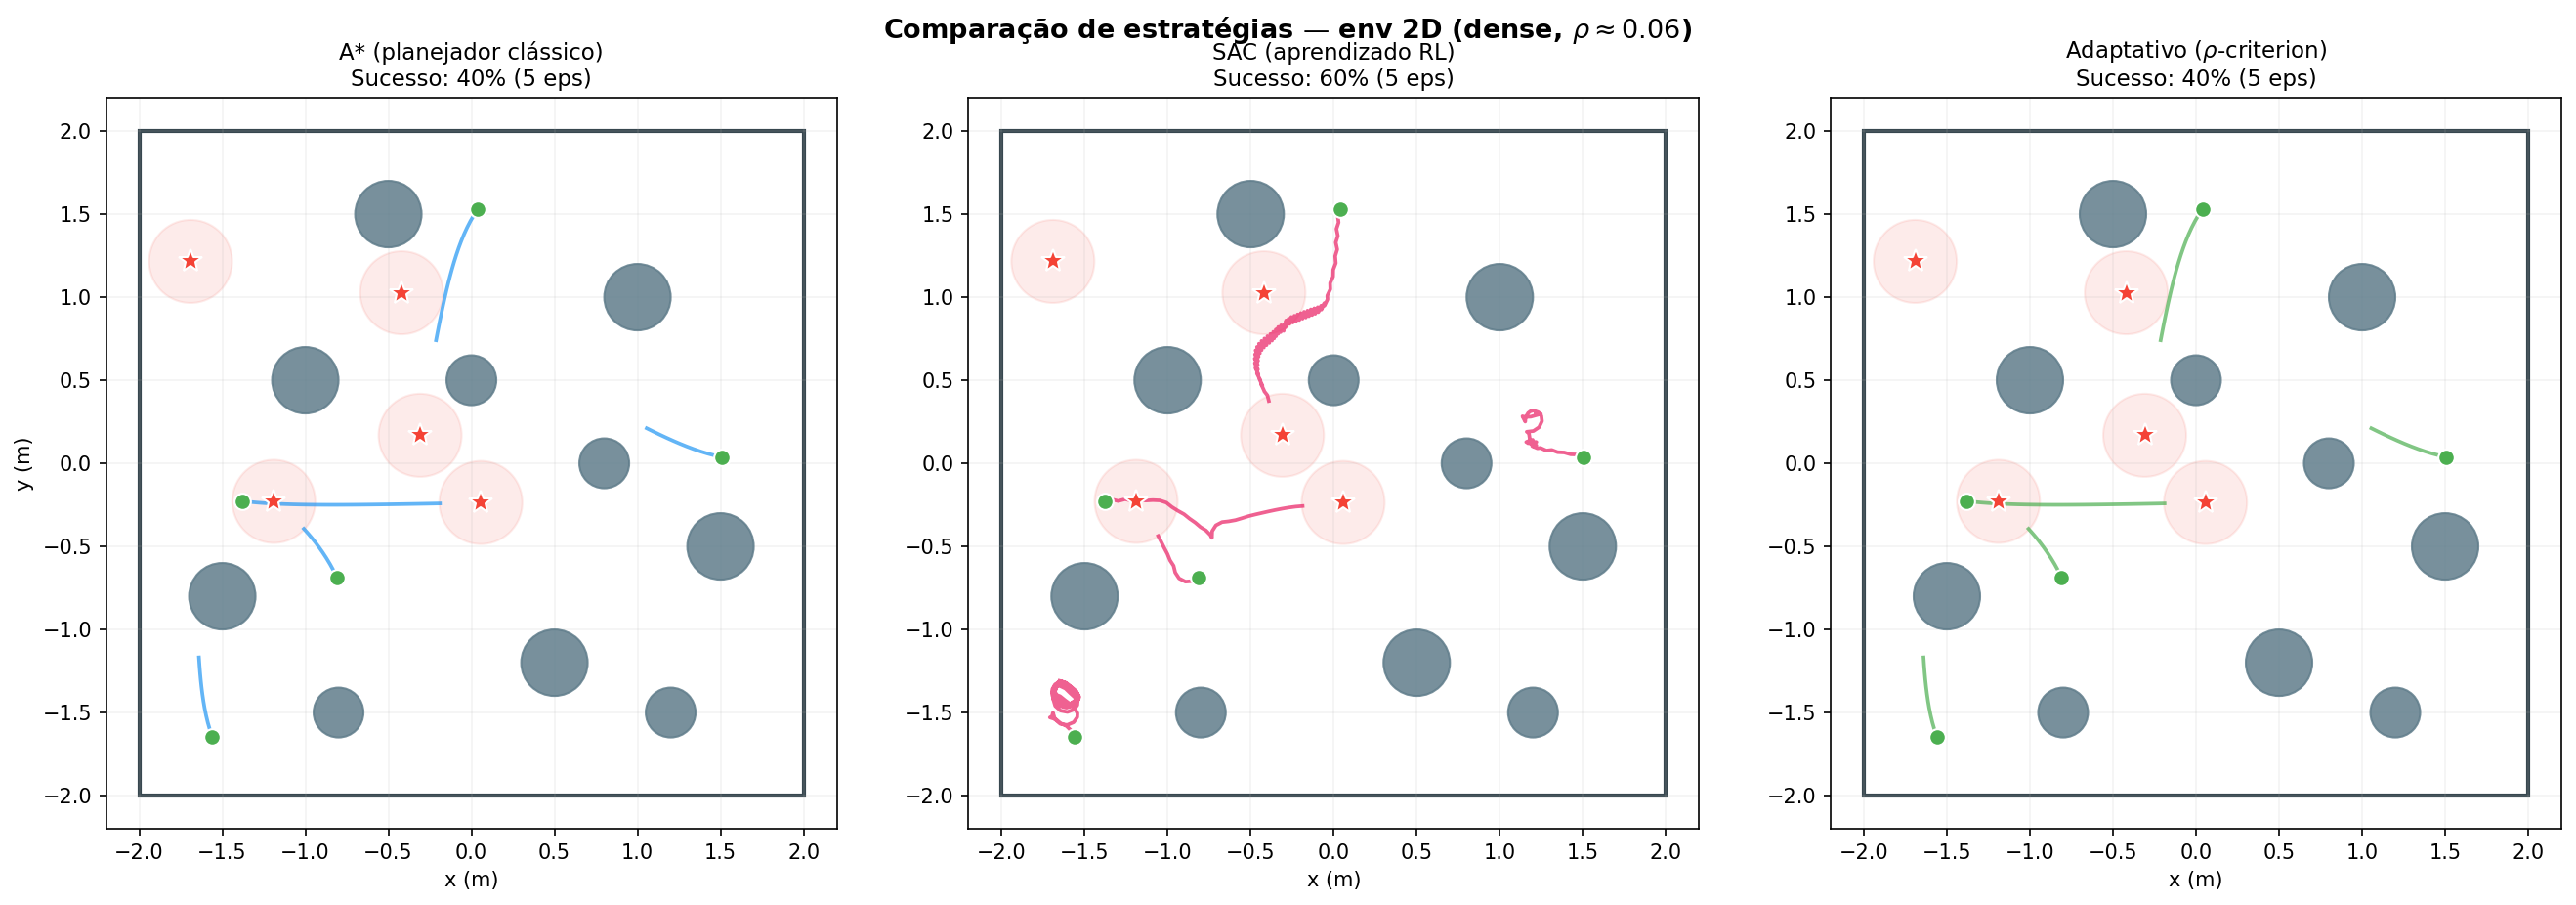
\includegraphics[width=\textwidth]{figs/2d/fig_2d_compare_dense.png}
    \caption{Trajetórias A* vs SAC vs Adaptativo}
  \end{subfigure}
  \caption{$\rho$-criterion em ação no ambiente denso ($\rho{\approx}0{,}35$). O critério
           ativa o SAC apenas nas regiões congestionadas, economizando inferência neural
           nas regiões livres. Validado em ambiente 2D leve (851$\times$ mais rápido que Gazebo).}
  \label{fig:2d_conpeex}
\end{figure}

% ── Figura 3: Degradação multi-agente (dados reais) ──────────
\begin{figure}[H]
  \centering
  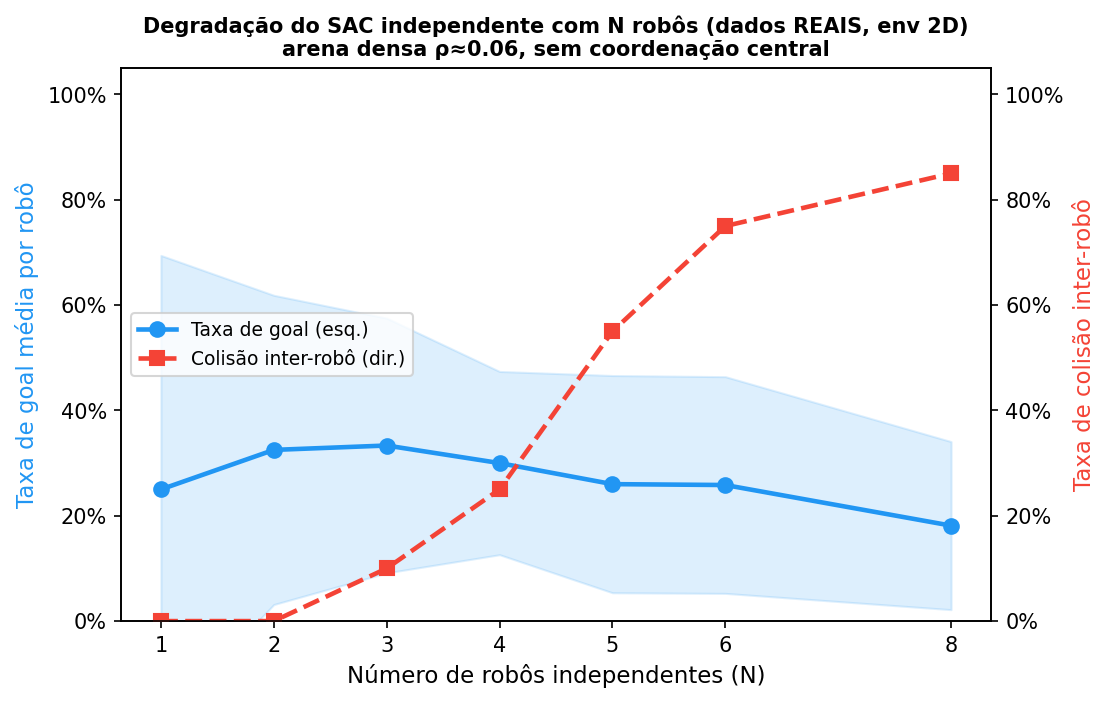
\includegraphics[width=\textwidth]{figs/marl/fig_marl_motivation_degradation_2d.png}
  \caption{Degradação empírica de N robôs SAC independentes (\textbf{dados reais}, env 2D).
           Colisão inter-robô sobe de 0\% ($N{=}1$) para 85\% ($N{=}8$): políticas
           independentes não garantem coordenação --- motivação para MARL como Fase 3.}
  \label{fig:marl_conpeex}
\end{figure}

% ── Figura 4: Curva de aprendizado ───────────────────────────
\begin{figure}[H]
  \centering
  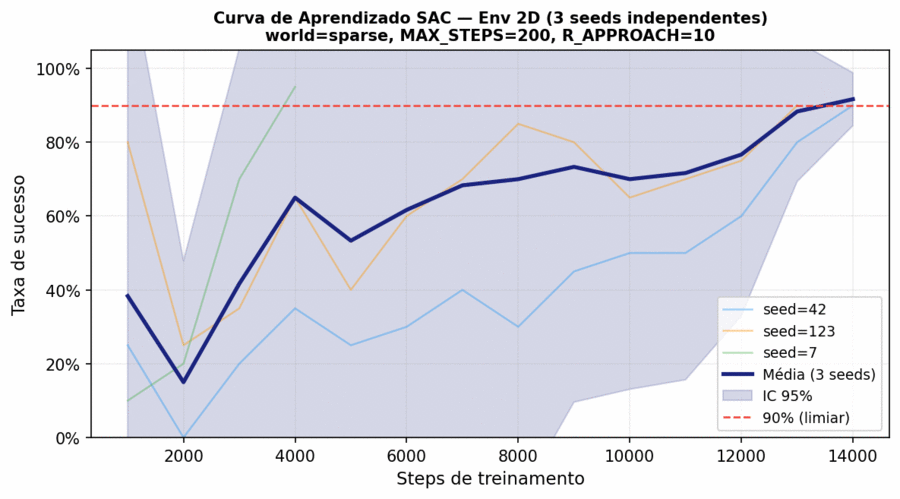
\includegraphics[width=0.85\textwidth]{figs/2d/fig_2d_learning_curve_ci.png}
  \caption{Curva de aprendizado SAC no env 2D (média $\pm$ IC~95\%, 3 seeds independentes):
           90\% de taxa de sucesso em 4.000--14.000 passos (6--13 min). Reprodutível em
           múltiplas seeds; permite iteração rápida de reward antes do ciclo lento do Gazebo.}
  \label{fig:learning_conpeex}
\end{figure}

\vspace{0.5cm}
\noindent\rule{\linewidth}{0.4pt}

% ── Checklist de submissão ───────────────────────────────────
\vspace{0.3cm}
\noindent\textbf{Checklist de submissão no PLATEIA:}

\begin{itemize}
  \item[$\square$] Login em \url{https://23conpeex.plateia.ufg.br/}
  \item[$\square$] Modalidade: \textbf{Seminário de Iniciação à Pesquisa --- PIP --- Iniciação Científica (IC)}
  \item[$\square$] Título colado em CAIXA ALTA (116 chars, dentro do limite de 150)
  \item[$\square$] Resumo colado e contagem de caracteres verificada (1.500--2.500)
  \item[$\square$] 5 palavras-chave inseridas individualmente
  \item[$\square$] Área: \textbf{Ciências Exatas, da Terra e Engenharias}
  \item[$\square$] Orientador: Prof. Dr. Aldo André Diaz Salazar --- INF/UFG
  \item[$\square$] Comprovante de submissão salvo
\end{itemize}

\vfill
\noindent\small\textit{Prazo: 26/06/2026 às 17h. Yan submete manualmente no PLATEIA.}

\end{document}
